\documentclass[journal,twoside,web]{ieeecolor}
\usepackage{generic}
\usepackage{cite}
\usepackage{amsmath,amssymb,amsfonts}
\usepackage{algorithmic}
\usepackage{graphicx}
\usepackage{textcomp}


\usepackage{multirow}



\def\BibTeX{{\rm B\kern-.05em{\sc i\kern-.025em b}\kern-.08em
    T\kern-.1667em\lower.7ex\hbox{E}\kern-.125emX}}
\markboth{\journalname, VOL. XX, NO. XX, XXXX 2017}
{Author \MakeLowercase{\textit{et al.}}: Point-process based representation learning for Electronic Health Records}
\begin{document}
\title{Point-process based representation learning for Electronic Health Records}
\author{Hojjat Karami, \IEEEmembership{Fellow, IEEE}, Anisoara Ionescu, and David Atienza, \IEEEmembership{Member, IEEE}
\thanks{This paragraph of the first footnote will contain the date on 
which you submitted your paper for review. It will also contain support 
information, including sponsor and financial support acknowledgment. For 
example, ``This work was supported in part by the U.S. Department of 
Commerce under Grant BS123456.'' }
\thanks{The next few paragraphs should contain 
the authors' current affiliations, including current address and e-mail. For 
example, F. A. Author is with the National Institute of Standards and 
Technology, Boulder, CO 80305 USA (e-mail: author@boulder.nist.gov). }
\thanks{S. B. Author, Jr., was with Rice University, Houston, TX 77005 USA. He is 
now with the Department of Physics, Colorado State University, Fort Collins, 
CO 80523 USA (e-mail: author@lamar.colostate.edu).}
\thanks{T. C. Author is with 
the Electrical Engineering Department, University of Colorado, Boulder, CO 
80309 USA, on leave from the National Research Institute for Metals, 
Tsukuba, Japan (e-mail: author@nrim.go.jp).}}

\maketitle


\begin{abstract}
    It is very well accepted that missingness in electronic health records (EHRs) are not at random which is regarded as informative missingness. The clinician’s decision on when to observe lab tests over time can be modeled using point processes. We propose a novel framework based on neural point process to analyze laboratory tests of ICU patients. This framework can take into account additional information for better characterization of conditional intensity function (CIF) as well as better accuracy in prediction of future timestamp and labels.
\end{abstract}

\begin{IEEEkeywords}
Enter keywords or phrases in alphabetical 
order, separated by commas. For a list of suggested keywords, send a blank 
e-mail to keywords@ieee.org or visit the site.
\end{IEEEkeywords}


\section{Introduction}
\label{sec:intro}

Writing an effective abstract is an indispensable part of any form of research, since it that can motivate the audience to read follow the rest of the text. In this task, I have analyzed five abstracts from the field of artificial intelligence (AI). The table in section 2 shows a summary of the most important aspects of the analyzed abstracts.



\section{Background}
\label{sec:Background}

\textbf{Temporal point process}

\textbf{Neural temporal point process}

\textbf{Handling irregular sampling}



\section{Related Works}
\label{sec:Related Works}

\section{Proposed Model}
\label{sec:Proposed Model}

Event sequence data consists of N sequences $\{\mathcal{S}_{i}\}_{i=1}^N$, where
 each sequence $\mathcal{S}_{i}$ is a series of $L_i$ events $\{ (t_j, e_j)
 \}_{j=1}^{L_i}$. Here, $e_j$ represents events that could be independent our mutually 
 exclusive occurring at $t_i$.
 \newline
 In addition to the event data, we might have additional information
  $\{\mathcal{D}_{i}\}_{i=1}^N$. Suppose that each state is represented as $\{
  (t_k, v_k, m_k) \}_{k=1}^{P_i}$, consisting of a time value $t_k\in
  \mathbb{R}^{+} $, an observed value  $z_k\in \mathbb{R} $ and a modality
  indicator  $m_k\in \{1, ..., M\} $.


\subsection{Event Encoder}
We use a similar transformer architecture [thp] for encoding events. The
advantage of the attention mechanism is that it discards recurrent architecture.
it is necessary to include temporal information. Similar to the original
positional encoding [vaswani], we use a temporal encoding procedure:


\begin{equation}\label{eq:1}
    [z(t_j)]_{k} = 
     \begin{cases} 
        \sin\left(  \frac{t_j}{\mathcal{T}^{(k-1)/d_t} }  \right) & \text{if } k \text{ is odd}\\
        \sin\left(  \frac{t_j}{\mathcal{T}^{k/d_t} }  \right) & \text{if } k \text{ is even}

        \end{cases} 
\end{equation} 





Here, $d_t \in \mathbb{N} $ is the dimensionality of encoded timestamp and $z
\in \mathbb{R}^{d_t} $ is the embeding vector of timestamp.

Each event mark $e_j$ is projected to a sparse binary vector representation. We
add an embedding layer to achieve a more compact and efficient representation
$emb$. Here, $w$ and $b$ are weights and biases of the embedding layer which can be
learned during network training. 

While previous works suggested adding temporal encoding to the embedded events,
we propose to concatenate these two vectors. The effectiveness of this
concatenation is further investigated in the results.

\begin{equation} x_{emb}=[y(k_j), z(t_j)] \end{equation}


Now that the $x_{emb}$ is ready for encoding, it is encoded through a standard
transformer encoder with multiple layers and attention heads.

\begin{equation}
    x_{enc}=TE(x_{emb})    
\end{equation}


\subsection{State Encoder}
Here, we propose a method to incorporate additional information for a
better representation. In healthcare, much data is available from different
modalities such as vital signs and laboratory values. 

Similar to [setF], we use an attention-based aggregation approach for encoding all additional information. Each side information  $ (t_k, v_k, m_k) $ can be represented by $s_k=(z(t_k), v_k, m_k)$. we define attention $a(\mathcal{S}_k,s_k )$

We define $\mathcal{S}_p$ to be the set of the first $p$ available information.
The goal is to calculate $a(\mathcal{S}_p,s_k ), k \leq p$ that is the relevance of $k$-th observation $s_k$ to the first $p$ observed values $\mathcal{S}_p$.
This is achieved by computing an embedding of the set elements using a smaller set functions $f^{\prime}$, and projecting the concatenation of the set representation and the individual set element into d-dimensional space:


\begin{align*}
    f^{\prime}(\mathcal{S}_p) = g^{\prime} \left(  \frac{1}{p} \sum_{s_k \in \mathcal{S}_p}  h^{\prime}_{\theta}(s_k) \right)  \\
    K_p=[f^{\prime}(\mathcal{S}_p), s_p]^T W^K   
\end{align*}

Furthermore, we define a query vector $w^q \in \mathbb{R}^d$, which allows the model to summarize different aspects of the dataset via

\begin{equation*}
    e_p=\frac{K_p.w^q}{\sqrt{d}  }
\end{equation*}

Now, the desired attention can be computed as follows:

\begin{equation*}
    a(\mathcal{S}_p,s_k)=\frac{\exp (e_p)}{\sum_{k\leq p} \exp (e_k)  } 
\end{equation*}

Finally, we compute a weighted aggregation of set elements:

\begin{equation*}
    f(\mathcal{S}_p) =     
    g_{\psi}\left(
    \sum_{s_k \in \mathcal{S}_p}  a(\mathcal{S}_p,s_k)h_{\theta}(s_k) 
    \right) 
\end{equation*}

Without loss of generality, we can consider multiple heads by adding an additional dimension to keys and queries.\\


All formulas are:

\begin{equation*}
    \begin{cases} 
f^{\prime}(\mathcal{S}_p) = g^{\prime} \left(   
 \frac{1}{p} \sum_{s_k \in \mathcal{S}_p}  h^{\prime}_{\theta}(s_k) 
\right) \\
K_p=[f^{\prime}(\mathcal{S}_p), s_p]^T W^K \\
e_p=\frac{K_p.w^q}{\sqrt{d}  }\\
a(\mathcal{S}_p,s_k)=\frac{\exp (e_p)}{\sum_{k\leq p} \exp (e_k)  } \\
f(\mathcal{S}_p) = \sum_{s_k \in \mathcal{S}_p}  a(\mathcal{S}_p,s_k)h_{\theta}(s_k) \\
    z_p=g_{\psi}\left(         f(\mathcal{S}_p)         \right) \\
    \end{cases} 
\end{equation*}


\subsection{Mark and Time Decoder}

by concatenating encoded events $x_{enc}$ and additional information $f^{\prime}(\mathcal{S}_p)$, we can predict next marks and times as follows:

\begin{equation}
    \hat{e}_{j+1}=MLP([x_j, f^{\prime}(\mathcal{S}_j)])
\end{equation}

\begin{equation}
    \hat{t}_{j+1}=MLP([x_j, f^{\prime}(\mathcal{S}_j)])
\end{equation}

\begin{equation}
    \mathcal{L}_{mark} =
\end{equation}
\begin{equation}
    \mathcal{L}_{time} = \sum_{j=1}^{L-1} \left(  (\hat{t}_{j+1}-t_j)-(t_{j+1}-t_j)  \right)^2
\end{equation}

\subsection{Event Decoder}
Once we obtain a representation of a patient using embedded events and states, we can try to parameterize conditional intensity functions (CIFs) of the events.

In neural point process literature, many approaches have been propose to decode either conditional or cumulative intensity function.

\begin{equation}
    \lambda_k(t|\mathcal{H}_t ) = f_k\left(\alpha_k \frac{t-t_j}{t_j}+\mathbf{w}_k^T \mathbf{x}_{enc}(t_j)+\mathbf{y}_k^T \mathbf{s}_{enc}(t_j) +b_k   \right)
\end{equation}

\begin{equation}
    \lambda_k(t|\mathcal{H}_t ) = f_k\left(\alpha_k \frac{t-t_j}{t_j}+\mathbf{w}_k^T \mathbf{x}_{enc}(t_j)+b_k   \right)
\end{equation}

\section{Experiments}
\label{sec:Experiments}

\subsection*{Datasets}

\textbf{Physionet 2019 Sepsis Early Prediction Challenge (\emph{P19})}.
This dataset contains clinical data of about 40k patients in ICU. Clinical data consist of demographics, vital signs and laboratory values as well as sepsis label in a one-hour time grid. Our objective is to predict the timestamp of next lab sampling events as well as measured variables (event marks) given the patient history.



% To show the effectiveness of the proposed method, we further consider the following scenarios:
% \begin{itemize}
%     \item Enc(Event)+Dec(NextEvent): Here
%     \item Enc(Event)+Dec(NextEvent+CIF): Here
%     \item Enc(Event+state)+Dec(NextEvent): Here
%     \item Enc(Event+state)+Dec(NextEvent+CIF): Here
% \end{itemize}




\textbf{MIMIC-IV (\emph{M4})}.
We selected Medical Information Mart for Intensive Care (MIMIC) IV [1], which is a real-world clinical database comprising health data relating to over 40,000 patients admitted to ICU at the Beth Israel Deaconess Medical Center.


\textbf{Synthea (\emph{Syn})}.
We used the Synthea simulator (Walonoski et al., 2018) which generates patient-level EHRs using human expert curated Markov processes. Here, we reused the already processed version of this data by Edgauard.


\textbf{Stackoverflow (\emph{SO})}.
StackOverflow is a question-answering website. The website rewards users with badges to promote engagement in the community, and the same badge can be rewarded multiple times to the same user. We collect data in a two-year period, and we treat each user’s reward history as a sequence. Each event in the sequence signifies receipt of a particular medal.


\subsection*{Scenarios}
To investigate the effectiveness of the proposed method, we consider three input scenarios (TE, DA, TE+DA) as well as three loss functions (next event, CIF, next event+CIF) which would result in nine scenarios.

The first series of experiments are conducted to investigate the advantage of encoding additional information for paramterization of intensity functions. We consider seven scenarios:
Here, the baseline models


To show the effectiveness of time concatenation we report.

\subsection*{Baselines}
we use NEURALTPP that is already developed pipeline by as they already considered a lot of comibinations.       

\subsection*{Metrics}
We report the weighted AUPRC, AUROC of next predicted event as well as root mean sqaure error (RMSE) of next measurement interval.
For evaluating the goodness of fit for the parameterized point process, we report normalized negative likelihood normalized by number of ocurred event (NLL/events). Furthermore, we can also evaluate the learned representation of each patient to predict the sepsis label in a binary classification task.

\section{Results and Discussion}
\label{sec:Results and Discussion}



% Please add the following required packages to your document preamble:
% \usepackage{multirow}
% \usepackage{graphicx}
\begin{table}[h!]
    \centering
    \caption{unsupervised learning}
    \label{tab:table1}
    \resizebox{\columnwidth}{!}{%    
    \begin{tabular}{cclllll}
    \hline
    \multirow{2}{*}{Dataset} & \multicolumn{2}{c}{Model}            & \multicolumn{2}{c}{next mark} & next time & CIFs  \\
                             & \multicolumn{1}{l}{module} & loss    & AUPRC         & AUROC         & RMSE      & NLL   \\ \hline
    \multirow{6}{*}{p12}     & \multirow{3}{*}{TE}        & MC      & 23.98         & 23.98         & 23.98     & 23.98 \\
                             &                            & ML      & 23.98         & 23.98         & 23.98     & 23.98 \\
                             &                            & SHPMARK & 23.98         & 23.98         & 23.98     & 23.98 \\
                             & \multirow{3}{*}{TEDA}      & MC      & 23.98         & 23.98         & 23.98     & 23.98 \\
                             &                            & ML      & 23.98         & 23.98         & 23.98     & 23.98 \\
                             &                            & SHPMARK & 23.98         & 23.98         & 23.98     & 23.98 \\ \hline
    \multirow{6}{*}{p19}     & \multirow{3}{*}{TE}        & MC      & 23.98         & 23.98         & 23.98     & 23.98 \\
                             &                            & ML      & 23.98         & 23.98         & 23.98     & 23.98 \\
                             &                            & SHPMARK & 23.98         & 23.98         & 23.98     & 23.98 \\
                             & \multirow{3}{*}{TEDA}      & MC      & 23.98         & 23.98         & 23.98     & 23.98 \\
                             &                            & ML      & 23.98         & 23.98         & 23.98     & 23.98 \\
                             &                            & SHPMARK & 23.98         & 23.98         & 23.98     & 23.98 \\ \hline
    \end{tabular}%
    }
\end{table}


% Please add the following required packages to your document preamble:
% \usepackage{multirow}
% \usepackage{graphicx}
\begin{table}[h!]

    \centering
    \caption{Transfer learnings}
    \label{tab:table2}
    \resizebox{\columnwidth}{!}{%
    \begin{tabular}{|cll|ll|ll|}
    \hline
    \multicolumn{3}{|c|}{model}                                                          & \multicolumn{2}{c|}{p12}           & \multicolumn{2}{c|}{p19}           \\ \hline
    \multicolumn{1}{|l|}{module}                & \multicolumn{1}{l|}{loss}    & freezed & \multicolumn{1}{l|}{AUPRC} & AUROC & \multicolumn{1}{l|}{AUPRC} & AUROC \\ \hline
    \multicolumn{1}{|c|}{\multirow{3}{*}{TE}}   & \multicolumn{1}{l|}{MC}      &         & \multicolumn{1}{l|}{23.98} & 23.98 & \multicolumn{1}{l|}{23.98} & 23.98 \\ \cline{2-7} 
    \multicolumn{1}{|c|}{}                      & \multicolumn{1}{l|}{ML}      &         & \multicolumn{1}{l|}{23.98} & 23.98 & \multicolumn{1}{l|}{23.98} & 23.98 \\ \cline{2-7} 
    \multicolumn{1}{|c|}{}                      & \multicolumn{1}{l|}{SHPMARK} &         & \multicolumn{1}{l|}{23.98} & 23.98 & \multicolumn{1}{l|}{23.98} & 23.98 \\ \hline
    \multicolumn{1}{|c|}{\multirow{3}{*}{TEDA}} & \multicolumn{1}{l|}{MC}      &         & \multicolumn{1}{l|}{23.98} & 23.98 & \multicolumn{1}{l|}{23.98} & 23.98 \\ \cline{2-7} 
    \multicolumn{1}{|c|}{}                      & \multicolumn{1}{l|}{ML}      &         & \multicolumn{1}{l|}{23.98} & 23.98 & \multicolumn{1}{l|}{23.98} & 23.98 \\ \cline{2-7} 
    \multicolumn{1}{|c|}{}                      & \multicolumn{1}{l|}{SHPMARK} &         & \multicolumn{1}{l|}{23.98} & 23.98 & \multicolumn{1}{l|}{23.98} & 23.98 \\ \hline
    \end{tabular}%
    }
    \end{table}


\subsection{Next event prediction}

using CIF does not seem to improve the next mark and time prediction.
this is new insight as previous studies has claimed this loss to be useful.


\subsection{Learned representation}

using CIF loss function leads to a better representation for sepsis.



\subsection{Likelihood estimation}

Although CIF does not imporve mark prediction, it has led to better representation of patient for downstream task such as sepsis prediction.

In addition, we can interprete some of learned CIF patterns.

explain the effect of time concatenation in SO dataset

\subsection{Model interpretability}


one advantage of proposed method is use of attention mechanisms in both event and state encoder.

tsne of learned representation. 4 modes:


\begin{itemize}
    \item (DA,TE)->(Mark, CIF)
\end{itemize}

attention of DA for sepsis prediction

attention matrix of events for SO dataset

\section{Conclusion}
\label{sec:Conclusion}








\section{Introduction}
\label{sec:introduction}
\IEEEPARstart{T}{his} document is a template for \LaTeX. If you are 
reading a paper or PDF version of this document, please download the 
electronic file, trans\_jour.tex, from the IEEE Web site at \underline
{http://www.ieee.org/authortools/trans\_jour.tex} so you can use it to prepare your manuscript. If 
you would prefer to use LaTeX, download IEEE's LaTeX style and sample files 
from the same Web page. You can also explore using the Overleaf editor at 
\underline
{https://www.overleaf.com/blog/278-how-to-use-overleaf-with-}\discretionary{}{}{}\underline
{ieee-collabratec-your-quick-guide-to-getting-started\#.}\discretionary{}{}{}\underline{xsVp6tpPkrKM9}

If your paper is intended for a conference, please contact your conference 
editor concerning acceptable word processor formats for your particular 
conference. 

IEEE will do the final formatting of your paper. If your paper is intended 
for a conference, please observe the conference page limits. 

\subsection{Abbreviations and Acronyms}
Define abbreviations and acronyms the first time they are used in the text, 
even after they have already been defined in the abstract. Abbreviations 
such as IEEE, SI, ac, and dc do not have to be defined. Abbreviations that 
incorporate periods should not have spaces: write ``C.N.R.S.,'' not ``C. N. 
R. S.'' Do not use abbreviations in the title unless they are unavoidable 
(for example, ``IEEE'' in the title of this article).

\subsection{Other Recommendations}
Use one space after periods and colons. Hyphenate complex modifiers: 
``zero-field-cooled magnetization.'' Avoid dangling participles, such as, 
``Using \eqref{eq}, the potential was calculated.'' [It is not clear who or what 
used \eqref{eq}.] Write instead, ``The potential was calculated by using \eqref{eq},'' or 
``Using \eqref{eq}, we calculated the potential.''

Use a zero before decimal points: ``0.25,'' not ``.25.'' Use 
``cm$^{3}$,'' not ``cc.'' Indicate sample dimensions as ``0.1 cm 
$\times $ 0.2 cm,'' not ``0.1 $\times $ 0.2 cm$^{2}$.'' The 
abbreviation for ``seconds'' is ``s,'' not ``sec.'' Use 
``Wb/m$^{2}$'' or ``webers per square meter,'' not 
``webers/m$^{2}$.'' When expressing a range of values, write ``7 to 
9'' or ``7--9,'' not ``7$\sim $9.''

A parenthetical statement at the end of a sentence is punctuated outside of 
the closing parenthesis (like this). (A parenthetical sentence is punctuated 
within the parentheses.) In American English, periods and commas are within 
quotation marks, like ``this period.'' Other punctuation is ``outside''! 
Avoid contractions; for example, write ``do not'' instead of ``don't.'' The 
serial comma is preferred: ``A, B, and C'' instead of ``A, B and C.''

If you wish, you may write in the first person singular or plural and use 
the active voice (``I observed that $\ldots$'' or ``We observed that $\ldots$'' 
instead of ``It was observed that $\ldots$''). Remember to check spelling. If 
your native language is not English, please get a native English-speaking 
colleague to carefully proofread your paper.

Try not to use too many typefaces in the same article. You're writing
scholarly papers, not ransom notes. Also please remember that MathJax
can't handle really weird typefaces.

\subsection{Equations}
Number equations consecutively with equation numbers in parentheses flush 
with the right margin, as in \eqref{eq}. To make your equations more 
compact, you may use the solidus (~/~), the exp function, or appropriate 
exponents. Use parentheses to avoid ambiguities in denominators. Punctuate 
equations when they are part of a sentence, as in
\begin{equation}E=mc^2.\label{eq}\end{equation}

Be sure that the symbols in your equation have been defined before the 
equation appears or immediately following. Italicize symbols ($T$ might refer 
to temperature, but T is the unit tesla). Refer to ``\eqref{eq},'' not ``Eq. \eqref{eq}'' 
or ``equation \eqref{eq},'' except at the beginning of a sentence: ``Equation \eqref{eq} 
is $\ldots$ .''

\subsection{\LaTeX-Specific Advice}

Please use ``soft'' (e.g., \verb|\eqref{Eq}|) cross references instead
of ``hard'' references (e.g., \verb|(1)|). That will make it possible
to combine sections, add equations, or change the order of figures or
citations without having to go through the file line by line.

Please don't use the \verb|{eqnarray}| equation environment. Use
\verb|{align}| or \verb|{IEEEeqnarray}| instead. The \verb|{eqnarray}|
environment leaves unsightly spaces around relation symbols.

Please note that the \verb|{subequations}| environment in {\LaTeX}
will increment the main equation counter even when there are no
equation numbers displayed. If you forget that, you might write an
article in which the equation numbers skip from (17) to (20), causing
the copy editors to wonder if you've discovered a new method of
counting.

{\BibTeX} does not work by magic. It doesn't get the bibliographic
data from thin air but from .bib files. If you use {\BibTeX} to produce a
bibliography you must send the .bib files. 

{\LaTeX} can't read your mind. If you assign the same label to a
subsubsection and a table, you might find that Table I has been cross
referenced as Table IV-B3. 

{\LaTeX} does not have precognitive abilities. If you put a
\verb|\label| command before the command that updates the counter it's
supposed to be using, the label will pick up the last counter to be
cross referenced instead. In particular, a \verb|\label| command
should not go before the caption of a figure or a table.

Do not use \verb|\nonumber| inside the \verb|{array}| environment. It
will not stop equation numbers inside \verb|{array}| (there won't be
any anyway) and it might stop a wanted equation number in the
surrounding equation.

If you are submitting your paper to a colorized journal, you can use
the following two lines at the start of the article to ensure its
appearance resembles the final copy:

\smallskip\noindent
\begin{small}
\begin{tabular}{l}
\verb+\+\texttt{documentclass[journal,twoside,web]\{ieeecolor\}}\\
\verb+\+\texttt{usepackage\{\textit{Journal\_Name}\}}
\end{tabular}
\end{small}










\section{Units}
Use either SI (MKS) or CGS as primary units. (SI units are strongly 
encouraged.) English units may be used as secondary units (in parentheses). 
This applies to papers in data storage. For example, write ``15 
Gb/cm$^{2}$ (100 Gb/in$^{2})$.'' An exception is when 
English units are used as identifiers in trade, such as ``3\textonehalf-in 
disk drive.'' Avoid combining SI and CGS units, such as current in amperes 
and magnetic field in oersteds. This often leads to confusion because 
equations do not balance dimensionally. If you must use mixed units, clearly 
state the units for each quantity in an equation.

The SI unit for magnetic field strength $H$ is A/m. However, if you wish to use 
units of T, either refer to magnetic flux density $B$ or magnetic field 
strength symbolized as $\mu _{0}H$. Use the center dot to separate 
compound units, e.g., ``A$\cdot $m$^{2}$.''

\section{Some Common Mistakes}
The word ``data'' is plural, not singular. The subscript for the 
permeability of vacuum $\mu _{0}$ is zero, not a lowercase letter 
``o.'' The term for residual magnetization is ``remanence''; the adjective 
is ``remanent''; do not write ``remnance'' or ``remnant.'' Use the word 
``micrometer'' instead of ``micron.'' A graph within a graph is an 
``inset,'' not an ``insert.'' The word ``alternatively'' is preferred to the 
word ``alternately'' (unless you really mean something that alternates). Use 
the word ``whereas'' instead of ``while'' (unless you are referring to 
simultaneous events). Do not use the word ``essentially'' to mean 
``approximately'' or ``effectively.'' Do not use the word ``issue'' as a 
euphemism for ``problem.'' When compositions are not specified, separate 
chemical symbols by en-dashes; for example, ``NiMn'' indicates the 
intermetallic compound Ni$_{0.5}$Mn$_{0.5}$ whereas 
``Ni--Mn'' indicates an alloy of some composition 
Ni$_{x}$Mn$_{1-x}$.

\begin{figure}[!t]
\centerline{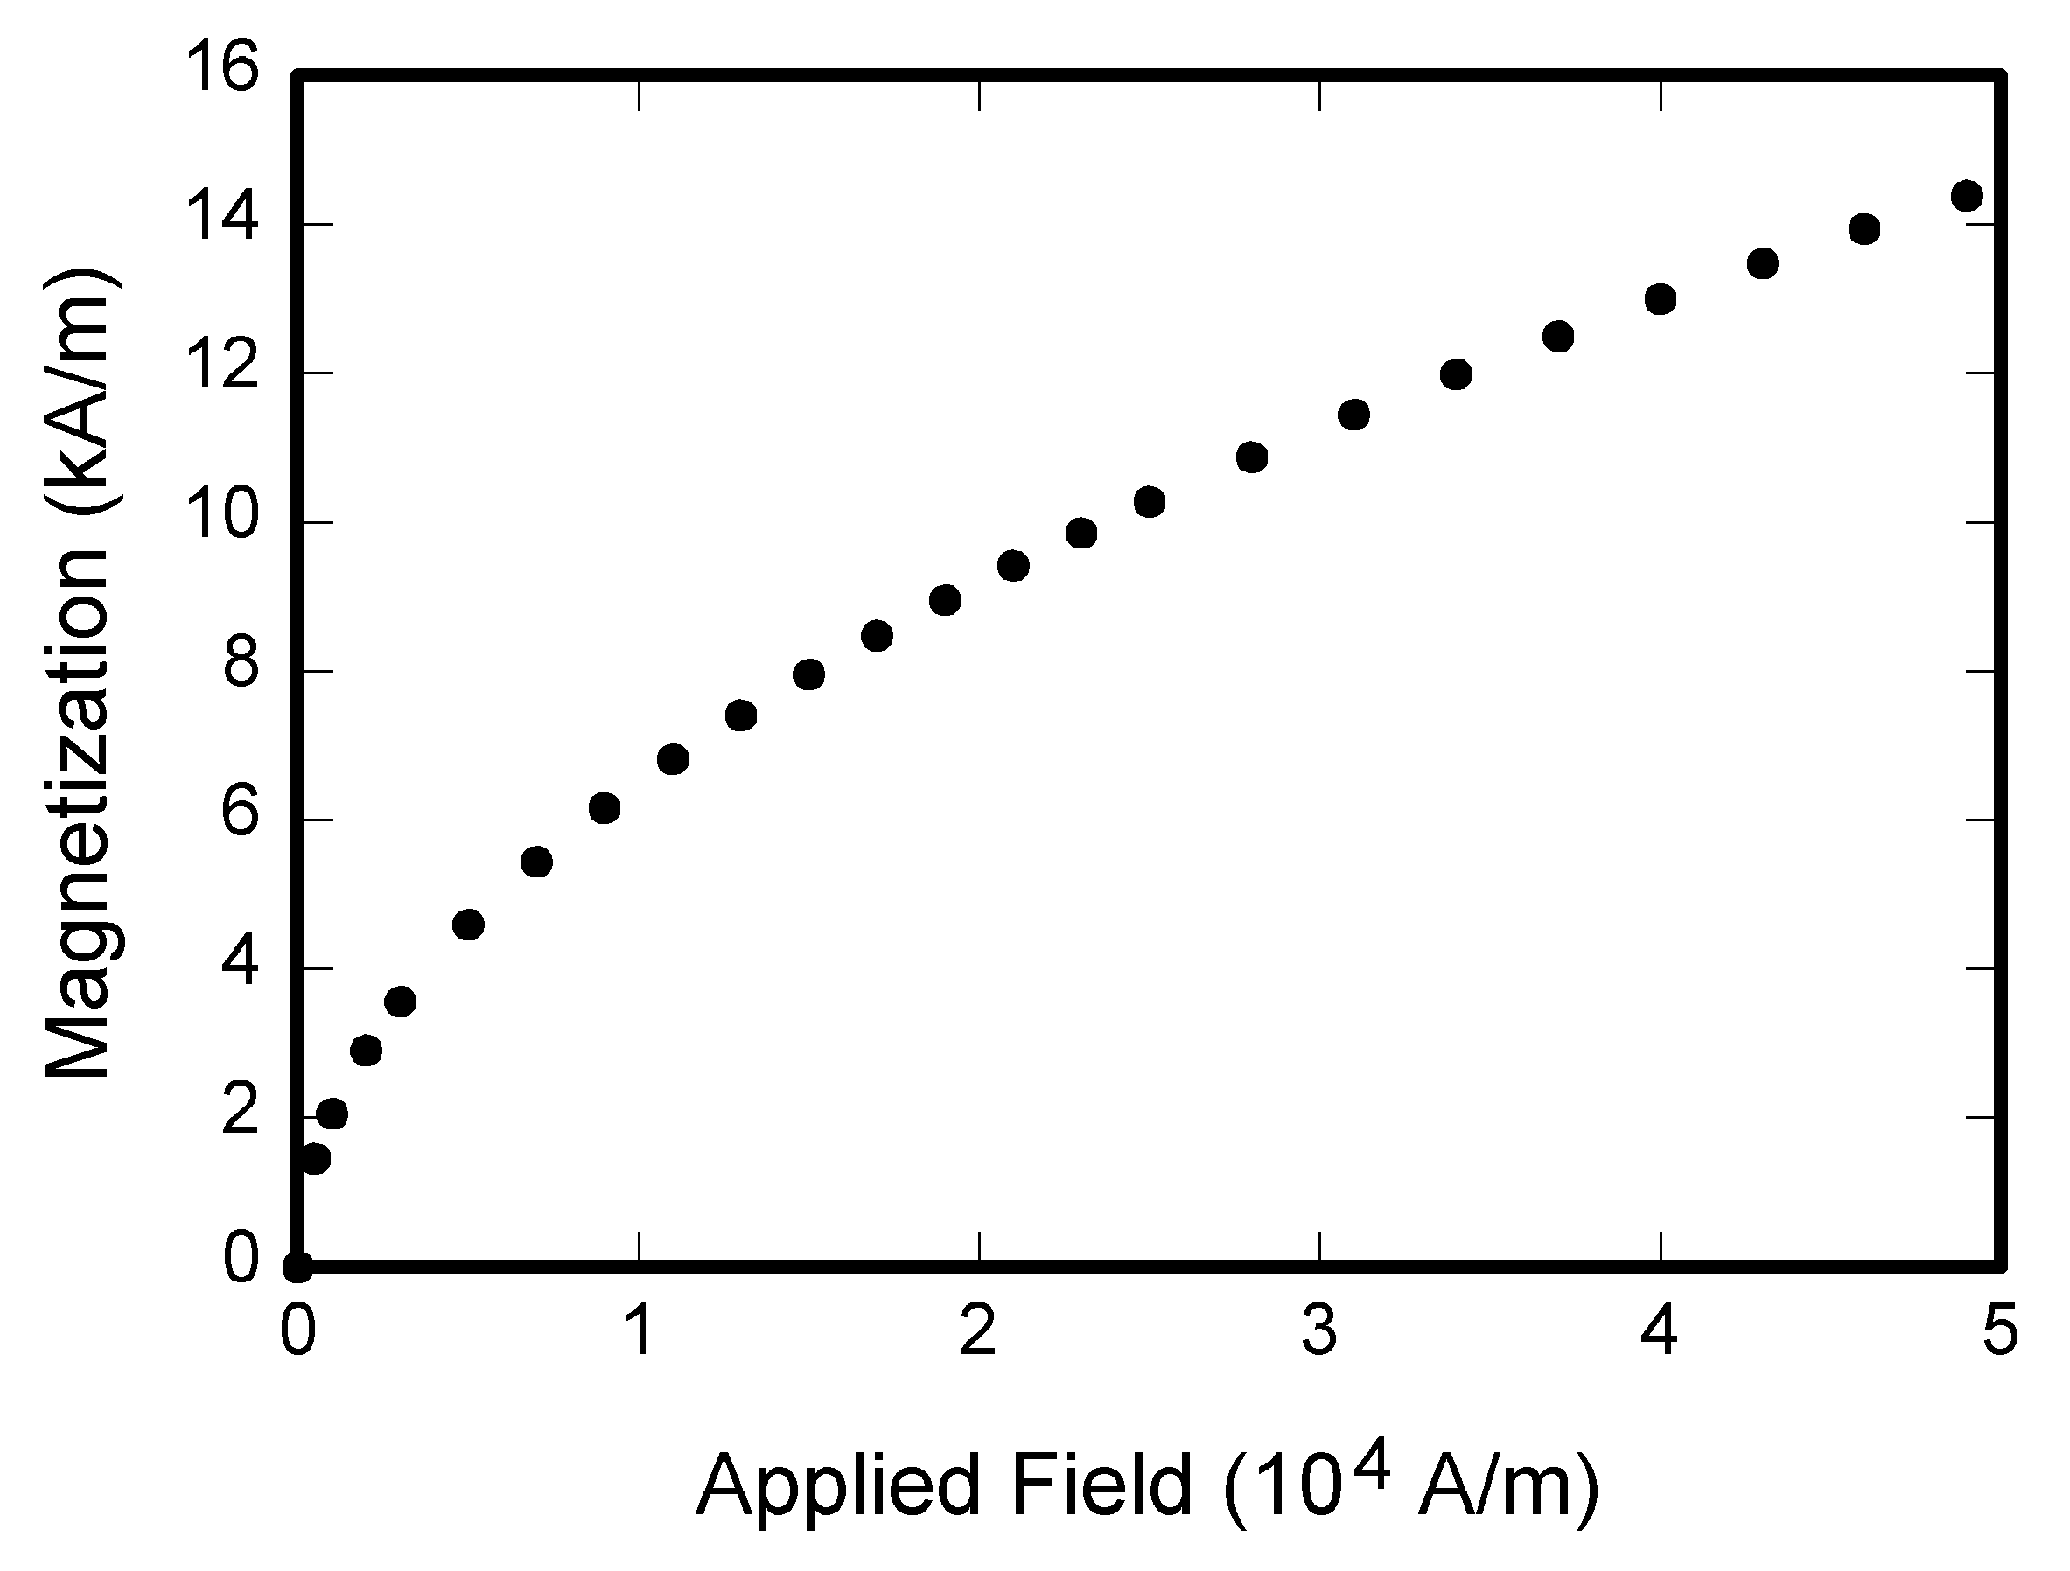
\includegraphics[width=\columnwidth]{fig1.png}}
\caption{Magnetization as a function of applied field.
It is good practice to explain the significance of the figure in the caption.}
\label{fig1}
\end{figure}

Be aware of the different meanings of the homophones ``affect'' (usually a 
verb) and ``effect'' (usually a noun), ``complement'' and ``compliment,'' 
``discreet'' and ``discrete,'' ``principal'' (e.g., ``principal 
investigator'') and ``principle'' (e.g., ``principle of measurement''). Do 
not confuse ``imply'' and ``infer.'' 

Prefixes such as ``non,'' ``sub,'' ``micro,'' ``multi,'' and ``ultra'' are 
not independent words; they should be joined to the words they modify, 
usually without a hyphen. There is no period after the ``et'' in the Latin 
abbreviation ``\emph{et al.}'' (it is also italicized). The abbreviation ``i.e.,'' means 
``that is,'' and the abbreviation ``e.g.,'' means ``for example'' (these 
abbreviations are not italicized).

A general IEEE styleguide is available at \underline{http://www.ieee.org/authortools}.

\section{Guidelines for Graphics Preparation and Submission}
\label{sec:guidelines}

\subsection{Types of Graphics}
The following list outlines the different types of graphics published in 
IEEE journals. They are categorized based on their construction, and use of 
color/shades of gray:

\subsubsection{Color/Grayscale figures}
{Figures that are meant to appear in color, or shades of black/gray. Such 
figures may include photographs, illustrations, multicolor graphs, and 
flowcharts.}

\subsubsection{Line Art figures}
{Figures that are composed of only black lines and shapes. These figures 
should have no shades or half-tones of gray, only black and white.}

\subsubsection{Author photos}
{Head and shoulders shots of authors that appear at the end of our papers. }

\subsubsection{Tables}
{Data charts which are typically black and white, but sometimes include 
color.}

\begin{table}
\caption{Units for Magnetic Properties}
\label{table}
\setlength{\tabcolsep}{3pt}
\begin{tabular}{|p{25pt}|p{75pt}|p{115pt}|}
\hline
Symbol& 
Quantity& 
Conversion from Gaussian and \par CGS EMU to SI $^{\mathrm{a}}$ \\
\hline
$\Phi $& 
magnetic flux& 
1 Mx $\to  10^{-8}$ Wb $= 10^{-8}$ V$\cdot $s \\
$B$& 
magnetic flux density, \par magnetic induction& 
1 G $\to  10^{-4}$ T $= 10^{-4}$ Wb/m$^{2}$ \\
$H$& 
magnetic field strength& 
1 Oe $\to  10^{3}/(4\pi )$ A/m \\
$m$& 
magnetic moment& 
1 erg/G $=$ 1 emu \par $\to 10^{-3}$ A$\cdot $m$^{2} = 10^{-3}$ J/T \\
$M$& 
magnetization& 
1 erg/(G$\cdot $cm$^{3}) =$ 1 emu/cm$^{3}$ \par $\to 10^{3}$ A/m \\
4$\pi M$& 
magnetization& 
1 G $\to  10^{3}/(4\pi )$ A/m \\
$\sigma $& 
specific magnetization& 
1 erg/(G$\cdot $g) $=$ 1 emu/g $\to $ 1 A$\cdot $m$^{2}$/kg \\
$j$& 
magnetic dipole \par moment& 
1 erg/G $=$ 1 emu \par $\to 4\pi \times  10^{-10}$ Wb$\cdot $m \\
$J$& 
magnetic polarization& 
1 erg/(G$\cdot $cm$^{3}) =$ 1 emu/cm$^{3}$ \par $\to 4\pi \times  10^{-4}$ T \\
$\chi , \kappa $& 
susceptibility& 
1 $\to  4\pi $ \\
$\chi_{\rho }$& 
mass susceptibility& 
1 cm$^{3}$/g $\to  4\pi \times  10^{-3}$ m$^{3}$/kg \\
$\mu $& 
permeability& 
1 $\to  4\pi \times  10^{-7}$ H/m \par $= 4\pi \times  10^{-7}$ Wb/(A$\cdot $m) \\
$\mu_{r}$& 
relative permeability& 
$\mu \to \mu_{r}$ \\
$w, W$& 
energy density& 
1 erg/cm$^{3} \to  10^{-1}$ J/m$^{3}$ \\
$N, D$& 
demagnetizing factor& 
1 $\to  1/(4\pi )$ \\
\hline
\multicolumn{3}{p{251pt}}{Vertical lines are optional in tables. Statements that serve as captions for 
the entire table do not need footnote letters. }\\
\multicolumn{3}{p{251pt}}{$^{\mathrm{a}}$Gaussian units are the same as cg emu for magnetostatics; Mx 
$=$ maxwell, G $=$ gauss, Oe $=$ oersted; Wb $=$ weber, V $=$ volt, s $=$ 
second, T $=$ tesla, m $=$ meter, A $=$ ampere, J $=$ joule, kg $=$ 
kilogram, H $=$ henry.}
\end{tabular}
\label{tab1}
\end{table}

\subsection{Multipart figures}
Figures compiled of more than one sub-figure presented side-by-side, or 
stacked. If a multipart figure is made up of multiple figure
types (one part is lineart, and another is grayscale or color) the figure 
should meet the stricter guidelines.

\subsection{File Formats For Graphics}\label{formats}
Format and save your graphics using a suitable graphics processing program 
that will allow you to create the images as PostScript (PS), Encapsulated 
PostScript (.EPS), Tagged Image File Format (.TIFF), Portable Document 
Format (.PDF), Portable Network Graphics (.PNG), or Metapost (.MPS), sizes them, and adjusts 
the resolution settings. When 
submitting your final paper, your graphics should all be submitted 
individually in one of these formats along with the manuscript.

\subsection{Sizing of Graphics}
Most charts, graphs, and tables are one column wide (3.5 inches/88 
millimeters/21 picas) or page wide (7.16 inches/181 millimeters/43 
picas). The maximum depth a graphic can be is 8.5 inches (216 millimeters/54
picas). When choosing the depth of a graphic, please allow space for a 
caption. Figures can be sized between column and page widths if the author 
chooses, however it is recommended that figures are not sized less than 
column width unless when necessary. 

There is currently one publication with column measurements that do not 
coincide with those listed above. Proceedings of the IEEE has a column 
measurement of 3.25 inches (82.5 millimeters/19.5 picas). 

The final printed size of author photographs is exactly
1 inch wide by 1.25 inches tall (25.4 millimeters$\,\times\,$31.75 millimeters/6 
picas$\,\times\,$7.5 picas). Author photos printed in editorials measure 1.59 inches 
wide by 2 inches tall (40 millimeters$\,\times\,$50 millimeters/9.5 picas$\,\times\,$12 
picas).

\subsection{Resolution }
The proper resolution of your figures will depend on the type of figure it 
is as defined in the ``Types of Figures'' section. Author photographs, 
color, and grayscale figures should be at least 300dpi. Line art, including 
tables should be a minimum of 600dpi.

\subsection{Vector Art}
In order to preserve the figures' integrity across multiple computer 
platforms, we accept files in the following formats: .EPS/.PDF/.PS. All 
fonts must be embedded or text converted to outlines in order to achieve the 
best-quality results.

\subsection{Color Space}
The term color space refers to the entire sum of colors that can be 
represented within the said medium. For our purposes, the three main color 
spaces are Grayscale, RGB (red/green/blue) and CMYK 
(cyan/magenta/yellow/black). RGB is generally used with on-screen graphics, 
whereas CMYK is used for printing purposes.

All color figures should be generated in RGB or CMYK color space. Grayscale 
images should be submitted in Grayscale color space. Line art may be 
provided in grayscale OR bitmap colorspace. Note that ``bitmap colorspace'' 
and ``bitmap file format'' are not the same thing. When bitmap color space 
is selected, .TIF/.TIFF/.PNG are the recommended file formats.

\subsection{Accepted Fonts Within Figures}
When preparing your graphics IEEE suggests that you use of one of the 
following Open Type fonts: Times New Roman, Helvetica, Arial, Cambria, and 
Symbol. If you are supplying EPS, PS, or PDF files all fonts must be 
embedded. Some fonts may only be native to your operating system; without 
the fonts embedded, parts of the graphic may be distorted or missing.

A safe option when finalizing your figures is to strip out the fonts before 
you save the files, creating ``outline'' type. This converts fonts to 
artwork what will appear uniformly on any screen.

\subsection{Using Labels Within Figures}

\subsubsection{Figure Axis labels }
Figure axis labels are often a source of confusion. Use words rather than 
symbols. As an example, write the quantity ``Magnetization,'' or 
``Magnetization M,'' not just ``M.'' Put units in parentheses. Do not label 
axes only with units. As in Fig. 1, for example, write ``Magnetization 
(A/m)'' or ``Magnetization (A$\cdot$m$^{-1}$),'' not just ``A/m.'' Do not label axes with a ratio of quantities and 
units. For example, write ``Temperature (K),'' not ``Temperature/K.'' 

Multipliers can be especially confusing. Write ``Magnetization (kA/m)'' or 
``Magnetization (10$^{3}$ A/m).'' Do not write ``Magnetization 
(A/m)$\,\times\,$1000'' because the reader would not know whether the top 
axis label in Fig. 1 meant 16000 A/m or 0.016 A/m. Figure labels should be 
legible, approximately 8 to 10 point type.

\subsubsection{Subfigure Labels in Multipart Figures and Tables}
Multipart figures should be combined and labeled before final submission. 
Labels should appear centered below each subfigure in 8 point Times New 
Roman font in the format of (a) (b) (c). 

\subsection{File Naming}
Figures (line artwork or photographs) should be named starting with the 
first 5 letters of the author's last name. The next characters in the 
filename should be the number that represents the sequential 
location of this image in your article. For example, in author 
``Anderson's'' paper, the first three figures would be named ander1.tif, 
ander2.tif, and ander3.ps.

Tables should contain only the body of the table (not the caption) and 
should be named similarly to figures, except that `.t' is inserted 
in-between the author's name and the table number. For example, author 
Anderson's first three tables would be named ander.t1.tif, ander.t2.ps, 
ander.t3.eps.

Author photographs should be named using the first five characters of the 
pictured author's last name. For example, four author photographs for a 
paper may be named: oppen.ps, moshc.tif, chen.eps, and duran.pdf.

If two authors or more have the same last name, their first initial(s) can 
be substituted for the fifth, fourth, third$\ldots$ letters of their surname 
until the degree where there is differentiation. For example, two authors 
Michael and Monica Oppenheimer's photos would be named oppmi.tif, and 
oppmo.eps.

\subsection{Referencing a Figure or Table Within Your Paper}
When referencing your figures and tables within your paper, use the 
abbreviation ``Fig.'' even at the beginning of a sentence. Do not abbreviate 
``Table.'' Tables should be numbered with Roman Numerals.

\subsection{Checking Your Figures: The IEEE Graphics Analyzer}
The IEEE Graphics Analyzer enables authors to pre-screen their graphics for 
compliance with IEEE Transactions and Journals standards before submission. 
The online tool, located at
\underline{http://graphicsqc.ieee.org/}, allows authors to 
upload their graphics in order to check that each file is the correct file 
format, resolution, size and colorspace; that no fonts are missing or 
corrupt; that figures are not compiled in layers or have transparency, and 
that they are named according to the IEEE Transactions and Journals naming 
convention. At the end of this automated process, authors are provided with 
a detailed report on each graphic within the web applet, as well as by 
email.

For more information on using the Graphics Analyzer or any other graphics 
related topic, contact the IEEE Graphics Help Desk by e-mail at 
graphics@ieee.org.

\subsection{Submitting Your Graphics}
Because IEEE will do the final formatting of your paper,
you do not need to position figures and tables at the top and bottom of each 
column. In fact, all figures, figure captions, and tables can be placed at 
the end of your paper. In addition to, or even in lieu of submitting figures 
within your final manuscript, figures should be submitted individually, 
separate from the manuscript in one of the file formats listed above in 
Section \ref{formats}. Place figure captions below the figures; place table titles 
above the tables. Please do not include captions as part of the figures, or 
put them in ``text boxes'' linked to the figures. Also, do not place borders 
around the outside of your figures.

\subsection{Color Processing/Printing in IEEE Journals}
All IEEE Transactions, Journals, and Letters allow an author to publish 
color figures on IEEE Xplore\textregistered\ at no charge, and automatically 
convert them to grayscale for print versions. In most journals, figures and 
tables may alternatively be printed in color if an author chooses to do so. 
Please note that this service comes at an extra expense to the author. If 
you intend to have print color graphics, include a note with your final 
paper indicating which figures or tables you would like to be handled that 
way, and stating that you are willing to pay the additional fee.

\section{Conclusion}
A conclusion section is not required. Although a conclusion may review the 
main points of the paper, do not replicate the abstract as the conclusion. A 
conclusion might elaborate on the importance of the work or suggest 
applications and extensions. 

\appendices

Appendixes, if needed, appear before the acknowledgment.

\section*{Acknowledgment}

The preferred spelling of the word ``acknowledgment'' in American English is 
without an ``e'' after the ``g.'' Use the singular heading even if you have 
many acknowledgments. Avoid expressions such as ``One of us (S.B.A.) would 
like to thank $\ldots$ .'' Instead, write ``F. A. Author thanks $\ldots$ .'' In most 
cases, sponsor and financial support acknowledgments are placed in the 
unnumbered footnote on the first page, not here.

\section*{References and Footnotes}

\subsection{References}
References need not be cited in text. When they are, they appear on the 
line, in square brackets, inside the punctuation. Multiple references are 
each numbered with separate brackets. When citing a section in a book, 
please give the relevant page numbers. In text, refer simply to the 
reference number. Do not use ``Ref.'' or ``reference'' except at the 
beginning of a sentence: ``Reference \cite{b3} shows $\ldots$ .'' Please do not use 
automatic endnotes in \emph{Word}, rather, type the reference list at the end of the 
paper using the ``References'' style.

Reference numbers are set flush left and form a column of their own, hanging 
out beyond the body of the reference. The reference numbers are on the line, 
enclosed in square brackets. In all references, the given name of the author 
or editor is abbreviated to the initial only and precedes the last name. Use 
them all; use \emph{et al.} only if names are not given. Use commas around Jr., 
Sr., and III in names. Abbreviate conference titles. When citing IEEE 
transactions, provide the issue number, page range, volume number, year, 
and/or month if available. When referencing a patent, provide the day and 
the month of issue, or application. References may not include all 
information; please obtain and include relevant information. Do not combine 
references. There must be only one reference with each number. If there is a 
URL included with the print reference, it can be included at the end of the 
reference. 

Other than books, capitalize only the first word in a paper title, except 
for proper nouns and element symbols. For papers published in translation 
journals, please give the English citation first, followed by the original 
foreign-language citation See the end of this document for formats and 
examples of common references. For a complete discussion of references and 
their formats, see the IEEE style manual at
\underline{http://www.ieee.org/authortools}.

\subsection{Footnotes}
Number footnotes separately in superscript numbers.\footnote{It is recommended that footnotes be avoided (except for 
the unnumbered footnote with the receipt date on the first page). Instead, 
try to integrate the footnote information into the text.} Place the actual 
footnote at the bottom of the column in which it is cited; do not put 
footnotes in the reference list (endnotes). Use letters for table footnotes 
(see Table \ref{table}).

\section{Submitting Your Paper for Review}

\subsection{Final Stage}
When you submit your final version (after your paper has been accepted), 
print it in two-column format, including figures and tables. You must also 
send your final manuscript on a disk, via e-mail, or through a Web 
manuscript submission system as directed by the society contact. You may use 
\emph{Zip} for large files, or compress files using \emph{Compress, Pkzip, Stuffit,} or \emph{Gzip.} 

Also, send a sheet of paper or PDF with complete contact information for all 
authors. Include full mailing addresses, telephone numbers, fax numbers, and 
e-mail addresses. This information will be used to send each author a 
complimentary copy of the journal in which the paper appears. In addition, 
designate one author as the ``corresponding author.'' This is the author to 
whom proofs of the paper will be sent. Proofs are sent to the corresponding 
author only.

\subsection{Review Stage Using ScholarOne\textregistered\ Manuscripts}
Contributions to the Transactions, Journals, and Letters may be submitted 
electronically on IEEE's on-line manuscript submission and peer-review 
system, ScholarOne\textregistered\ Manuscripts. You can get a listing of the 
publications that participate in ScholarOne at 
\underline{http://www.ieee.org/publications\_standards/publications/}\discretionary{}{}{}\underline{authors/authors\_submission.html}.
First check if you have an existing account. If there is none, please create 
a new account. After logging in, go to your Author Center and click ``Submit 
First Draft of a New Manuscript.'' 

Along with other information, you will be asked to select the subject from a 
pull-down list. Depending on the journal, there are various steps to the 
submission process; you must complete all steps for a complete submission. 
At the end of each step you must click ``Save and Continue''; just uploading 
the paper is not sufficient. After the last step, you should see a 
confirmation that the submission is complete. You should also receive an 
e-mail confirmation. For inquiries regarding the submission of your paper on 
ScholarOne Manuscripts, please contact oprs-support@ieee.org or call +1 732 
465 5861.

ScholarOne Manuscripts will accept files for review in various formats. 
Please check the guidelines of the specific journal for which you plan to 
submit.

You will be asked to file an electronic copyright form immediately upon 
completing the submission process (authors are responsible for obtaining any 
security clearances). Failure to submit the electronic copyright could 
result in publishing delays later. You will also have the opportunity to 
designate your article as ``open access'' if you agree to pay the IEEE open 
access fee. 

\subsection{Final Stage Using ScholarOne Manuscripts}
Upon acceptance, you will receive an email with specific instructions 
regarding the submission of your final files. To avoid any delays in 
publication, please be sure to follow these instructions. Most journals 
require that final submissions be uploaded through ScholarOne Manuscripts, 
although some may still accept final submissions via email. Final 
submissions should include source files of your accepted manuscript, high 
quality graphic files, and a formatted pdf file. If you have any questions 
regarding the final submission process, please contact the administrative 
contact for the journal. 

In addition to this, upload a file with complete contact information for all 
authors. Include full mailing addresses, telephone numbers, fax numbers, and 
e-mail addresses. Designate the author who submitted the manuscript on 
ScholarOne Manuscripts as the ``corresponding author.'' This is the only 
author to whom proofs of the paper will be sent. 

\subsection{Copyright Form}
Authors must submit an electronic IEEE Copyright Form (eCF) upon submitting 
their final manuscript files. You can access the eCF system through your 
manuscript submission system or through the Author Gateway. You are 
responsible for obtaining any necessary approvals and/or security 
clearances. For additional information on intellectual property rights, 
visit the IEEE Intellectual Property Rights department web page at 
\underline{http://www.ieee.org/publications\_standards/publications/rights/}\discretionary{}{}{}\underline{index.html}. 

\section{IEEE Publishing Policy}
The general IEEE policy requires that authors should only submit original 
work that has neither appeared elsewhere for publication, nor is under 
review for another refereed publication. The submitting author must disclose 
all prior publication(s) and current submissions when submitting a 
manuscript. Do not publish ``preliminary'' data or results. The submitting 
author is responsible for obtaining agreement of all coauthors and any 
consent required from employers or sponsors before submitting an article. 
The IEEE Transactions and Journals Department strongly discourages courtesy 
authorship; it is the obligation of the authors to cite only relevant prior 
work.

The IEEE Transactions and Journals Department does not publish conference 
records or proceedings, but can publish articles related to conferences that 
have undergone rigorous peer review. Minimally, two reviews are required for 
every article submitted for peer review.

\section{Publication Principles}
The two types of contents of that are published are; 1) peer-reviewed and 2) 
archival. The Transactions and Journals Department publishes scholarly 
articles of archival value as well as tutorial expositions and critical 
reviews of classical subjects and topics of current interest. 

Authors should consider the following points:

\begin{enumerate}
\item Technical papers submitted for publication must advance the state of knowledge and must cite relevant prior work. 
\item The length of a submitted paper should be commensurate with the importance, or appropriate to the complexity, of the work. For example, an obvious extension of previously published work might not be appropriate for publication or might be adequately treated in just a few pages.
\item Authors must convince both peer reviewers and the editors of the scientific and technical merit of a paper; the standards of proof are higher when extraordinary or unexpected results are reported. 
\item Because replication is required for scientific progress, papers submitted for publication must provide sufficient information to allow readers to perform similar experiments or calculations and 
use the reported results. Although not everything need be disclosed, a paper 
must contain new, useable, and fully described information. For example, a 
specimen's chemical composition need not be reported if the main purpose of 
a paper is to introduce a new measurement technique. Authors should expect 
to be challenged by reviewers if the results are not supported by adequate 
data and critical details.
\item Papers that describe ongoing work or announce the latest technical achievement, which are suitable for presentation at a professional conference, may not be appropriate for publication.
\end{enumerate}

\section{Reference Examples}

\begin{itemize}

\item \emph{Basic format for books:}\\
J. K. Author, ``Title of chapter in the book,'' in \emph{Title of His Published Book, x}th ed. City of Publisher, (only U.S. State), Country: Abbrev. of Publisher, year, ch. $x$, sec. $x$, pp. \emph{xxx--xxx.}\\
See \cite{b1,b2}.

\item \emph{Basic format for periodicals:}\\
J. K. Author, ``Name of paper,'' \emph{Abbrev. Title of Periodical}, vol. \emph{x, no}. $x, $pp\emph{. xxx--xxx, }Abbrev. Month, year, DOI. 10.1109.\emph{XXX}.123456.\\
See \cite{b3}--\cite{b5}.

\item \emph{Basic format for reports:}\\
J. K. Author, ``Title of report,'' Abbrev. Name of Co., City of Co., Abbrev. State, Country, Rep. \emph{xxx}, year.\\
See \cite{b6,b7}.

\item \emph{Basic format for handbooks:}\\
\emph{Name of Manual/Handbook, x} ed., Abbrev. Name of Co., City of Co., Abbrev. State, Country, year, pp. \emph{xxx--xxx.}\\
See \cite{b8,b9}.

\item \emph{Basic format for books (when available online):}\\
J. K. Author, ``Title of chapter in the book,'' in \emph{Title of
Published Book}, $x$th ed. City of Publisher, State, Country: Abbrev.
of Publisher, year, ch. $x$, sec. $x$, pp. \emph{xxx--xxx}. [Online].
Available: \underline{http://www.web.com}\\
See \cite{b10}--\cite{b13}.

\item \emph{Basic format for journals (when available online):}\\
J. K. Author, ``Name of paper,'' \emph{Abbrev. Title of Periodical}, vol. $x$, no. $x$, pp. \emph{xxx--xxx}, Abbrev. Month, year. Accessed on: Month, Day, year, DOI: 10.1109.\emph{XXX}.123456, [Online].\\
See \cite{b14}--\cite{b16}.

\item \emph{Basic format for papers presented at conferences (when available online): }\\
J.K. Author. (year, month). Title. presented at abbrev. conference title. [Type of Medium]. Available: site/path/file\\
See \cite{b17}.

\item \emph{Basic format for reports and handbooks (when available online):}\\
J. K. Author. ``Title of report,'' Company. City, State, Country. Rep. no., (optional: vol./issue), Date. [Online] Available: site/path/file\\
See \cite{b18,b19}.

\item \emph{Basic format for computer programs and electronic documents (when available online): }\\
Legislative body. Number of Congress, Session. (year, month day). \emph{Number of bill or resolution}, \emph{Title}. [Type of medium]. Available: site/path/file\\
\textbf{\emph{NOTE: }ISO recommends that capitalization follow the accepted practice for the language or script in which the information is given.}\\
See \cite{b20}.

\item \emph{Basic format for patents (when available online):}\\
Name of the invention, by inventor's name. (year, month day). Patent Number [Type of medium]. Available: site/path/file\\
See \cite{b21}.

\item \emph{Basic format}\emph{for conference proceedings (published):}\\
J. K. Author, ``Title of paper,'' in \emph{Abbreviated Name of Conf.}, City of Conf., Abbrev. State (if given), Country, year, pp. \emph{xxxxxx.}\\
See \cite{b22}.

\item \emph{Example for papers presented at conferences (unpublished):}\\
See \cite{b23}.

\item \emph{Basic format for patents}$:$\\
J. K. Author, ``Title of patent,'' U.S. Patent \emph{x xxx xxx}, Abbrev. Month, day, year.\\
See \cite{b24}.

\item \emph{Basic format for theses (M.S.) and dissertations (Ph.D.):}
\begin{enumerate}
\item J. K. Author, ``Title of thesis,'' M.S. thesis, Abbrev. Dept., Abbrev. Univ., City of Univ., Abbrev. State, year.
\item J. K. Author, ``Title of dissertation,'' Ph.D. dissertation, Abbrev. Dept., Abbrev. Univ., City of Univ., Abbrev. State, year.
\end{enumerate}
See \cite{b25,b26}.

\item \emph{Basic format for the most common types of unpublished references:}
\begin{enumerate}
\item J. K. Author, private communication, Abbrev. Month, year.
\item J. K. Author, ``Title of paper,'' unpublished.
\item J. K. Author, ``Title of paper,'' to be published.
\end{enumerate}
See \cite{b27}--\cite{b29}.

\item \emph{Basic formats for standards:}
\begin{enumerate}
\item \emph{Title of Standard}, Standard number, date.
\item \emph{Title of Standard}, Standard number, Corporate author, location, date.
\end{enumerate}
See \cite{b30,b31}.

\item \emph{Article number in~reference examples:}\\
See \cite{b32,b33}.

\item \emph{Example when using et al.:}\\
See \cite{b34}.

\end{itemize}

\begin{thebibliography}{00}

\bibitem{b1} G. O. Young, ``Synthetic structure of industrial plastics,'' in \emph{Plastics,} 2\textsuperscript{nd} ed., vol. 3, J. Peters, Ed. New York, NY, USA: McGraw-Hill, 1964, pp. 15--64.

\bibitem{b2} W.-K. Chen, \emph{Linear Networks and Systems.} Belmont, CA, USA: Wadsworth, 1993, pp. 123--135.

\bibitem{b3} J. U. Duncombe, ``Infrared navigation---Part I: An assessment of feasibility,'' \emph{IEEE Trans. Electron Devices}, vol. ED-11, no. 1, pp. 34--39, Jan. 1959, 10.1109/TED.2016.2628402.

\bibitem{b4} E. P. Wigner, ``Theory of traveling-wave optical laser,'' \emph{Phys. Rev}., vol. 134, pp. A635--A646, Dec. 1965.

\bibitem{b5} E. H. Miller, ``A note on reflector arrays,'' \emph{IEEE Trans. Antennas Propagat}., to be published.

\bibitem{b6} E. E. Reber, R. L. Michell, and C. J. Carter, ``Oxygen absorption in the earth's atmosphere,'' Aerospace Corp., Los Angeles, CA, USA, Tech. Rep. TR-0200 (4230-46)-3, Nov. 1988.

\bibitem{b7} J. H. Davis and J. R. Cogdell, ``Calibration program for the 16-foot antenna,'' Elect. Eng. Res. Lab., Univ. Texas, Austin, TX, USA, Tech. Memo. NGL-006-69-3, Nov. 15, 1987.

\bibitem{b8} \emph{Transmission Systems for Communications}, 3\textsuperscript{rd} ed., Western Electric Co., Winston-Salem, NC, USA, 1985, pp. 44--60.

\bibitem{b9} \emph{Motorola Semiconductor Data Manual}, Motorola Semiconductor Products Inc., Phoenix, AZ, USA, 1989.

\bibitem{b10} G. O. Young, ``Synthetic structure of industrial
plastics,'' in Plastics, vol. 3, Polymers of Hexadromicon, J. Peters,
Ed., 2\textsuperscript{nd} ed. New York, NY, USA: McGraw-Hill, 1964, pp. 15-64.
[Online]. Available:
\underline{http://www.bookref.com}.

\bibitem{b11} \emph{The Founders' Constitution}, Philip B. Kurland
and Ralph Lerner, eds., Chicago, IL, USA: Univ. Chicago Press, 1987.
[Online]. Available: \underline{http://press-pubs.uchicago.edu/founders/}

\bibitem{b12} The Terahertz Wave eBook. ZOmega Terahertz Corp., 2014.
[Online]. Available:
\underline{http://dl.z-thz.com/eBook/zomega\_ebook\_pdf\_1206\_sr.pdf}. Accessed on: May 19, 2014.

\bibitem{b13} Philip B. Kurland and Ralph Lerner, eds., \emph{The
Founders' Constitution.} Chicago, IL, USA: Univ. of Chicago Press,
1987, Accessed on: Feb. 28, 2010, [Online] Available:
\underline{http://press-pubs.uchicago.edu/founders/}

\bibitem{b14} J. S. Turner, ``New directions in communications,'' \emph{IEEE J. Sel. Areas Commun}., vol. 13, no. 1, pp. 11-23, Jan. 1995.

\bibitem{b15} W. P. Risk, G. S. Kino, and H. J. Shaw, ``Fiber-optic frequency shifter using a surface acoustic wave incident at an oblique angle,'' \emph{Opt. Lett.}, vol. 11, no. 2, pp. 115--117, Feb. 1986.

\bibitem{b16} P. Kopyt \emph{et al., ``}Electric properties of graphene-based conductive layers from DC up to terahertz range,'' \emph{IEEE THz Sci. Technol.,} to be published. DOI: 10.1109/TTHZ.2016.2544142.

\bibitem{b17} PROCESS Corporation, Boston, MA, USA. Intranets:
Internet technologies deployed behind the firewall for corporate
productivity. Presented at INET96 Annual Meeting. [Online].
Available: \underline{http://home.process.com/Intranets/wp2.htp}

\bibitem{b18} R. J. Hijmans and J. van Etten, ``Raster: Geographic analysis and modeling with raster data,'' R Package Version 2.0-12, Jan. 12, 2012. [Online]. Available: \underline {http://CRAN.R-project.org/package=raster} 

\bibitem{b19} Teralyzer. Lytera UG, Kirchhain, Germany [Online].
Available:
\underline{http://www.lytera.de/Terahertz\_THz\_Spectroscopy.php?id=home}, Accessed on: Jun. 5, 2014

\bibitem{b20} U.S. House. 102\textsuperscript{nd} Congress, 1\textsuperscript{st} Session. (1991, Jan. 11). \emph{H. Con. Res. 1, Sense of the Congress on Approval of}  \emph{Military Action}. [Online]. Available: LEXIS Library: GENFED File: BILLS

\bibitem{b21} Musical toothbrush with mirror, by L.M.R. Brooks. (1992, May 19). Patent D 326 189 [Online]. Available: NEXIS Library: LEXPAT File: DES

\bibitem{b22} D. B. Payne and J. R. Stern, ``Wavelength-switched pas- sively coupled single-mode optical network,'' in \emph{Proc. IOOC-ECOC,} Boston, MA, USA, 1985, pp. 585--590.

\bibitem{b23} D. Ebehard and E. Voges, ``Digital single sideband detection for interferometric sensors,'' presented at the \emph{2\textsuperscript{nd} Int. Conf. Optical Fiber Sensors,} Stuttgart, Germany, Jan. 2-5, 1984.

\bibitem{b24} G. Brandli and M. Dick, ``Alternating current fed power supply,'' U.S. Patent 4 084 217, Nov. 4, 1978.

\bibitem{b25} J. O. Williams, ``Narrow-band analyzer,'' Ph.D. dissertation, Dept. Elect. Eng., Harvard Univ., Cambridge, MA, USA, 1993.

\bibitem{b26} N. Kawasaki, ``Parametric study of thermal and chemical nonequilibrium nozzle flow,'' M.S. thesis, Dept. Electron. Eng., Osaka Univ., Osaka, Japan, 1993.

\bibitem{b27} A. Harrison, private communication, May 1995.

\bibitem{b28} B. Smith, ``An approach to graphs of linear forms,'' unpublished.

\bibitem{b29} A. Brahms, ``Representation error for real numbers in binary computer arithmetic,'' IEEE Computer Group Repository, Paper R-67-85.

\bibitem{b30} IEEE Criteria for Class IE Electric Systems, IEEE Standard 308, 1969.

\bibitem{b31} Letter Symbols for Quantities, ANSI Standard Y10.5-1968.

\bibitem{b32} R. Fardel, M. Nagel, F. Nuesch, T. Lippert, and A. Wokaun, ``Fabrication of organic light emitting diode pixels by laser-assisted forward transfer,'' \emph{Appl. Phys. Lett.}, vol. 91, no. 6, Aug. 2007, Art. no. 061103.~

\bibitem{b33} J. Zhang and N. Tansu, ``Optical gain and laser characteristics of InGaN quantum wells on ternary InGaN substrates,'' \emph{IEEE Photon. J.}, vol. 5, no. 2, Apr. 2013, Art. no. 2600111

\bibitem{b34} S. Azodolmolky~\emph{et al.}, Experimental demonstration of an impairment aware network planning and operation tool for transparent/translucent optical networks,''~\emph{J. Lightw. Technol.}, vol. 29, no. 4, pp. 439--448, Sep. 2011.

\end{thebibliography}

\begin{IEEEbiography}[{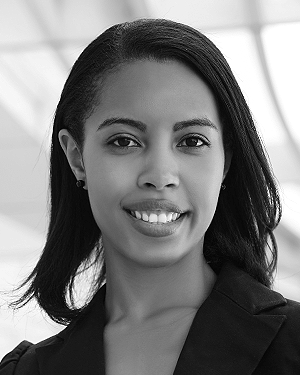
\includegraphics[width=1in,height=1.25in,clip,keepaspectratio]{a1.png}}]{First A. Author} (M'76--SM'81--F'87) and all authors may include 
biographies. Biographies are often not included in conference-related
papers. This author became a Member (M) of IEEE in 1976, a Senior
Member (SM) in 1981, and a Fellow (F) in 1987. The first paragraph may
contain a place and/or date of birth (list place, then date). Next,
the author's educational background is listed. The degrees should be
listed with type of degree in what field, which institution, city,
state, and country, and year the degree was earned. The author's major
field of study should be lower-cased. 

The second paragraph uses the pronoun of the person (he or she) and not the 
author's last name. It lists military and work experience, including summer 
and fellowship jobs. Job titles are capitalized. The current job must have a 
location; previous positions may be listed 
without one. Information concerning previous publications may be included. 
Try not to list more than three books or published articles. The format for 
listing publishers of a book within the biography is: title of book 
(publisher name, year) similar to a reference. Current and previous research 
interests end the paragraph. The third paragraph begins with the author's 
title and last name (e.g., Dr.\ Smith, Prof.\ Jones, Mr.\ Kajor, Ms.\ Hunter). 
List any memberships in professional societies other than the IEEE. Finally, 
list any awards and work for IEEE committees and publications. If a 
photograph is provided, it should be of good quality, and 
professional-looking. Following are two examples of an author's biography.
\end{IEEEbiography}

\begin{IEEEbiography}[{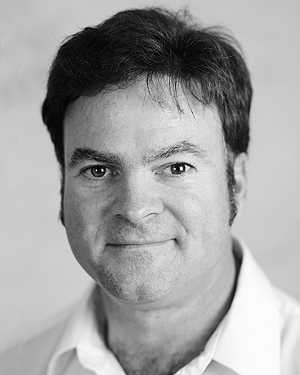
\includegraphics[width=1in,height=1.25in,clip,keepaspectratio]{a2.png}}]{Second B. Author} was born in Greenwich Village, New York, NY, USA in 
1977. He received the B.S. and M.S. degrees in aerospace engineering from 
the University of Virginia, Charlottesville, in 2001 and the Ph.D. degree in 
mechanical engineering from Drexel University, Philadelphia, PA, in 2008.

From 2001 to 2004, he was a Research Assistant with the Princeton Plasma 
Physics Laboratory. Since 2009, he has been an Assistant Professor with the 
Mechanical Engineering Department, Texas A{\&}M University, College Station. 
He is the author of three books, more than 150 articles, and more than 70 
inventions. His research interests include high-pressure and high-density 
nonthermal plasma discharge processes and applications, microscale plasma 
discharges, discharges in liquids, spectroscopic diagnostics, plasma 
propulsion, and innovation plasma applications. He is an Associate Editor of 
the journal \emph{Earth, Moon, Planets}, and holds two patents. 

Dr. Author was a recipient of the International Association of Geomagnetism 
and Aeronomy Young Scientist Award for Excellence in 2008, and the IEEE 
Electromagnetic Compatibility Society Best Symposium Paper Award in 2011. 
\end{IEEEbiography}

\begin{IEEEbiography}[{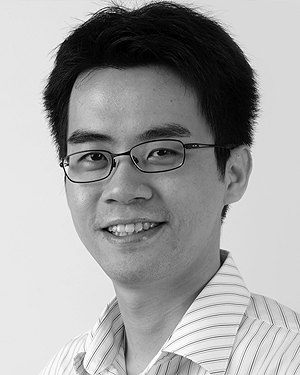
\includegraphics[width=1in,height=1.25in,clip,keepaspectratio]{a3.png}}]{Third C. Author, Jr.} (M'87) received the B.S. degree in mechanical 
engineering from National Chung Cheng University, Chiayi, Taiwan, in 2004 
and the M.S. degree in mechanical engineering from National Tsing Hua 
University, Hsinchu, Taiwan, in 2006. He is currently pursuing the Ph.D. 
degree in mechanical engineering at Texas A{\&}M University, College 
Station, TX, USA.

From 2008 to 2009, he was a Research Assistant with the Institute of 
Physics, Academia Sinica, Tapei, Taiwan. His research interest includes the 
development of surface processing and biological/medical treatment 
techniques using nonthermal atmospheric pressure plasmas, fundamental study 
of plasma sources, and fabrication of micro- or nanostructured surfaces. 

Mr. Author's awards and honors include the Frew Fellowship (Australian 
Academy of Science), the I. I. Rabi Prize (APS), the European Frequency and 
Time Forum Award, the Carl Zeiss Research Award, the William F. Meggers 
Award and the Adolph Lomb Medal (OSA).
\end{IEEEbiography}

\end{document}
